\section{Neutrino mass ordering sensitivity}
\label{sec:mh_sens}

In this section, the toy-throwing approach described in Section~\ref{sec:analysis_framework} is used to explore the neutrino mass ordering sensitivity as a function of exposure in detail. In all cases, a joint ND+FD fit is performed, and the reactor $\theta_{13}$ constraint is always applied, as described in Section~\ref{sec:analysis_framework}. An equal split between FHC and RHC running is assumed based on the results obtained in Section~\ref{sec:run_plan_opt}.

\begin{figure}[htbp]
  \centering
  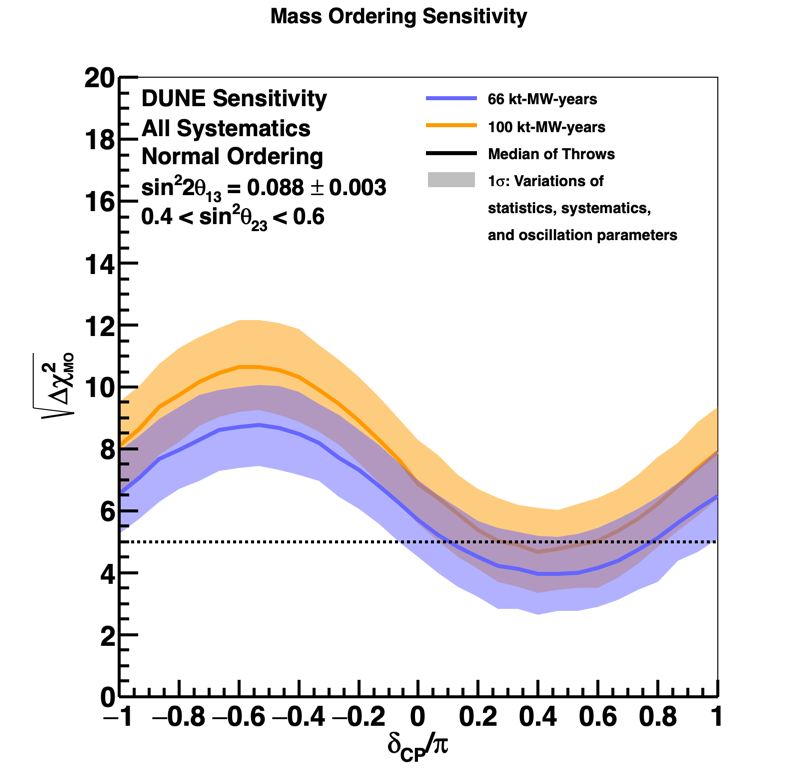
\includegraphics[width=1\linewidth, trim={0cm 0cm 0cm 2.3cm}, clip]{mh_two_exps_throws_nh_2019_v4_lowexp.png}
  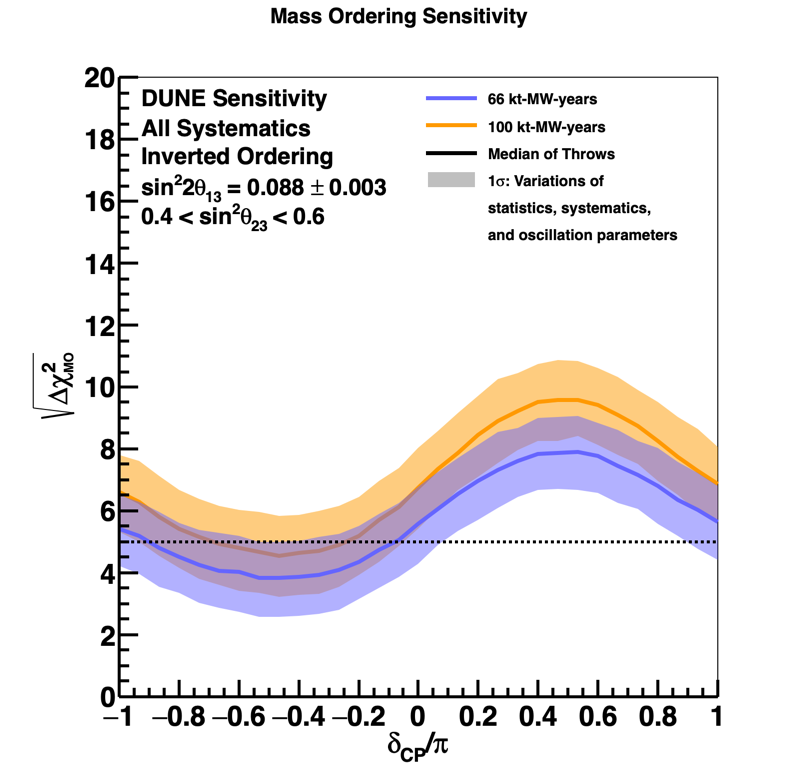
\includegraphics[width=1\linewidth, trim={0cm 0cm 0cm 2.3cm}, clip]{mh_two_exps_throws_ih_2019_v4_lowexp.png}
  \caption{Significance of the DUNE determination of the neutrino mass ordering, as a function of the true value of \deltacp, for 66 kt-MW-yr (blue) and 100 kt-MW-yr (orange) exposures. The width of the transparent bands cover 68\% of fits in which random throws are used to simulate systematic, oscillation parameter and statistical variations, with independent fits performed for each throw constrained by prior uncertainties. The solid lines show the median significance.}
  \label{fig:mh_bands}
\end{figure}
Figure~\ref{fig:mh_bands} shows the significance with which the neutrino mass ordering can be determined for both true NO and IO, for exposures of 66 and 100 kt-MW-yr. The sensitivity metric used is the square root of the difference between the best fit $\chi^{2}$ value obtained using each ordering, as shown in Equation~\ref{eq:mh_chi2}, which is calculated for each throw of the systematics, other oscillation parameters and statistics. The characteristic shape of the MH sensitivity in Figure~\ref{fig:mh_bands} results from near degeneracy between matter and CPV effects that occurs near $\deltacp=\pi/2$ ($\deltacp=-\pi/2$) for true normal (inverted) ordering. Dedicated studies have shown that special attention must be paid to the statistical interpretation of neutrino mass ordering sensitivities~\cite{Ciuffoli:2013rza,Qian:2012zn,Blennow:2013oma} because the \dchisqMO metric does not follow the expected chi-square distribution for one degree of freedom, so the interpretation of the $\sqrt{\dchisqMO}$ as the sensitivity is complicated.

\begin{figure*}[htbp]
  \centering
  \subfloat[6 kt-MW-yr]   {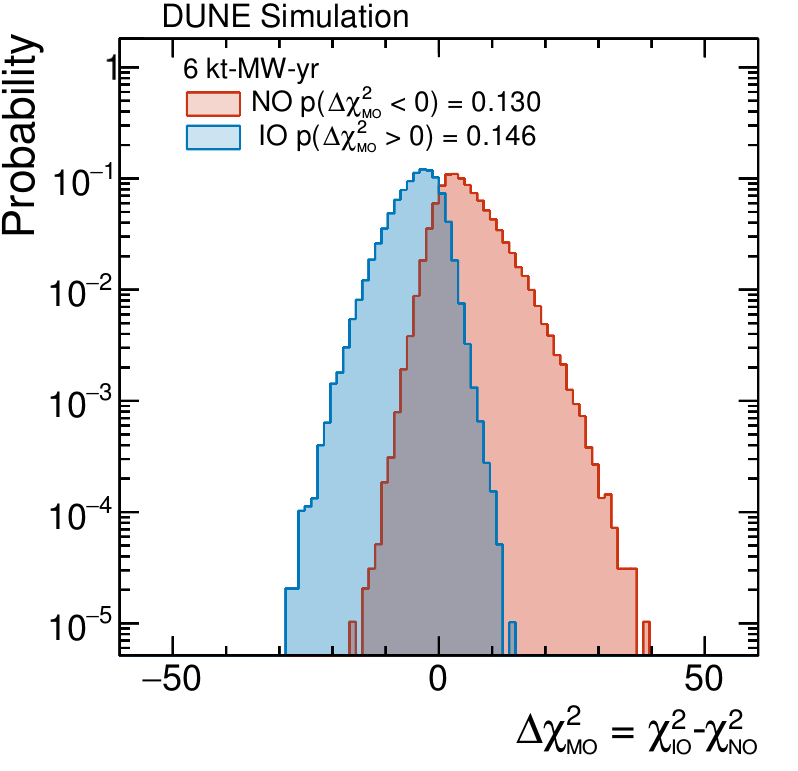
\includegraphics[width=0.33\linewidth]{MH_comp_ndfd_6ktMWyr_th13.png}}
  \subfloat[12 kt-MW-yr]  {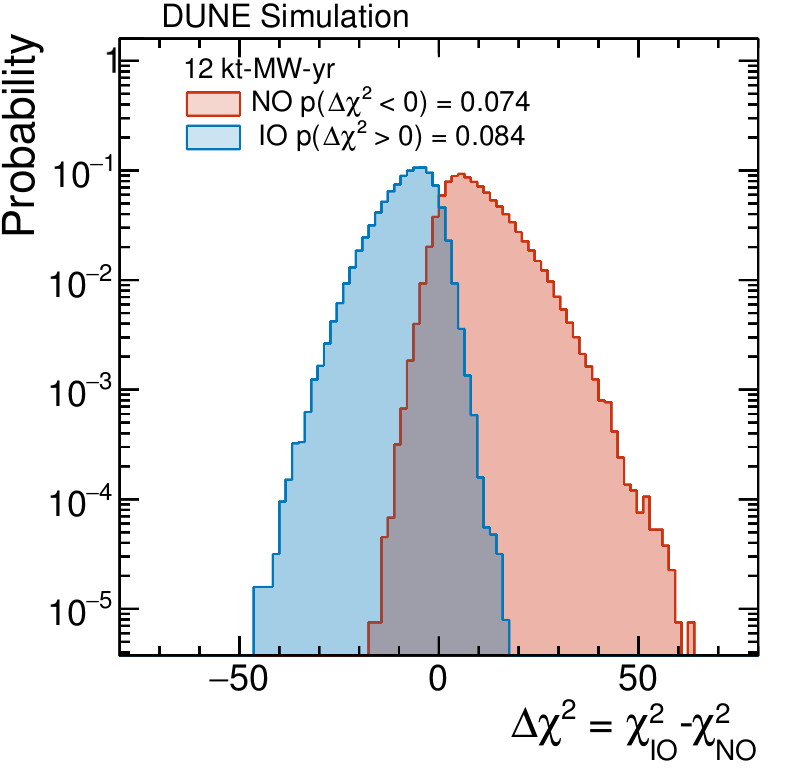
\includegraphics[width=0.33\linewidth]{MH_comp_ndfd_12ktMWyr_th13.png}}
  \subfloat[24 kt-MW-yr]  {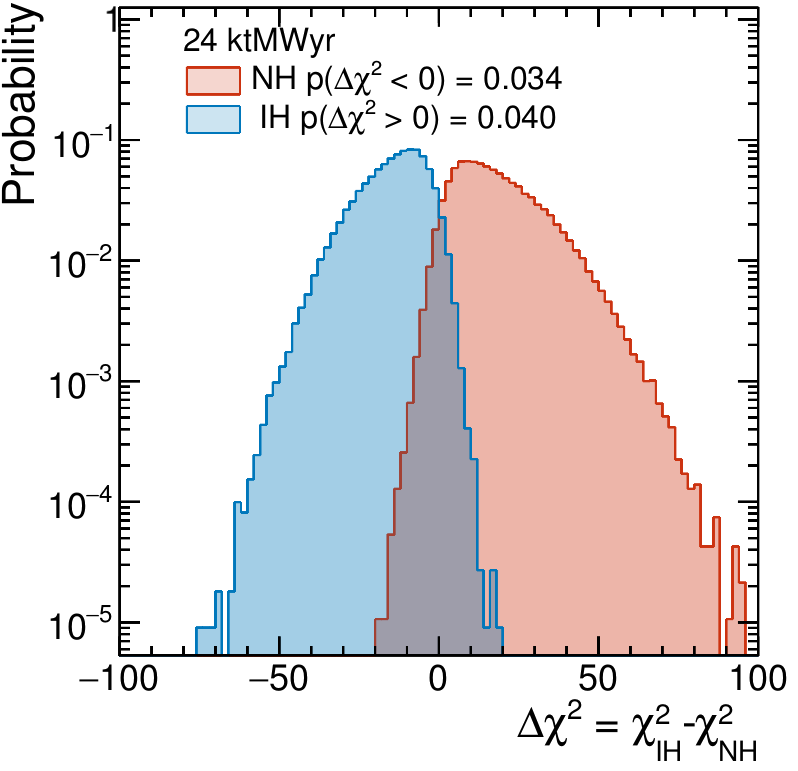
\includegraphics[width=0.33\linewidth]{MH_comp_ndfd_24ktMWyr_th13.png}}\\
  \subfloat[66 kt-MW-yr]  {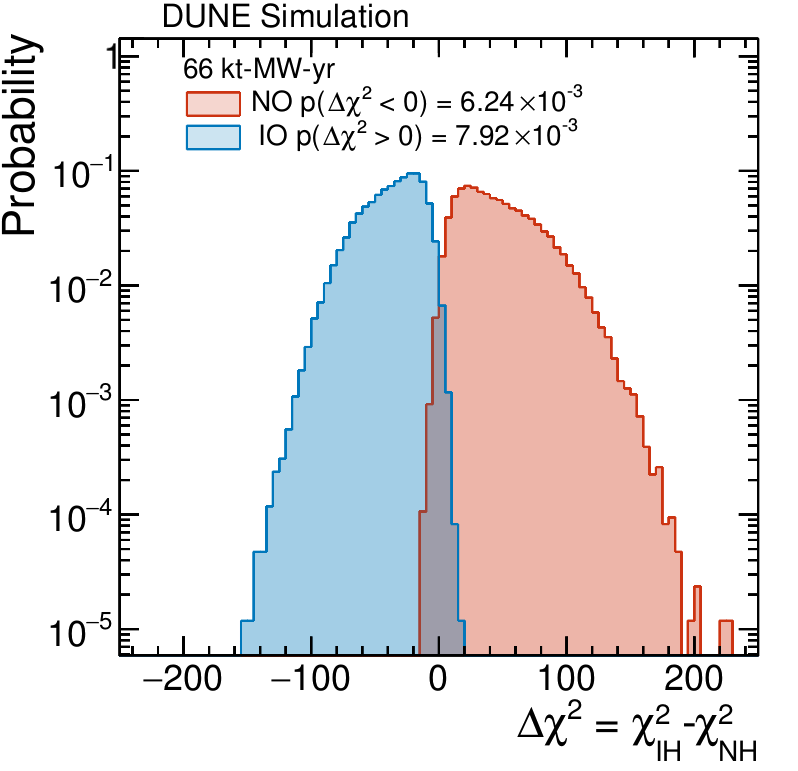
\includegraphics[width=0.33\linewidth]{MH_comp_ndfd_66ktMWyr_th13.png}}
  \subfloat[100 kt-MW-yr] {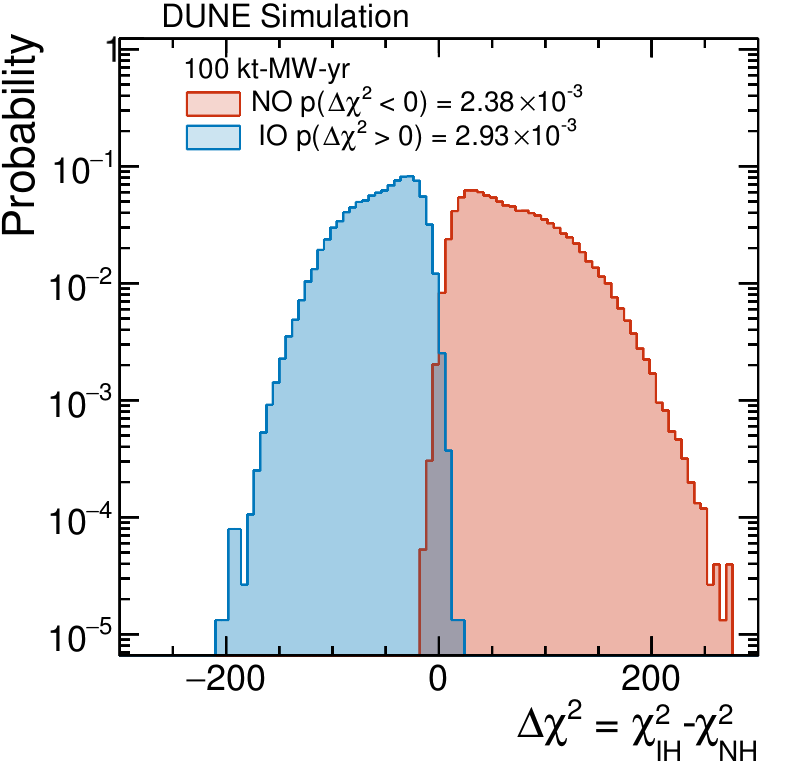
\includegraphics[width=0.33\linewidth]{MH_comp_ndfd_100ktMWyr_th13.png}}
  \subfloat[336 kt-MW-yr] {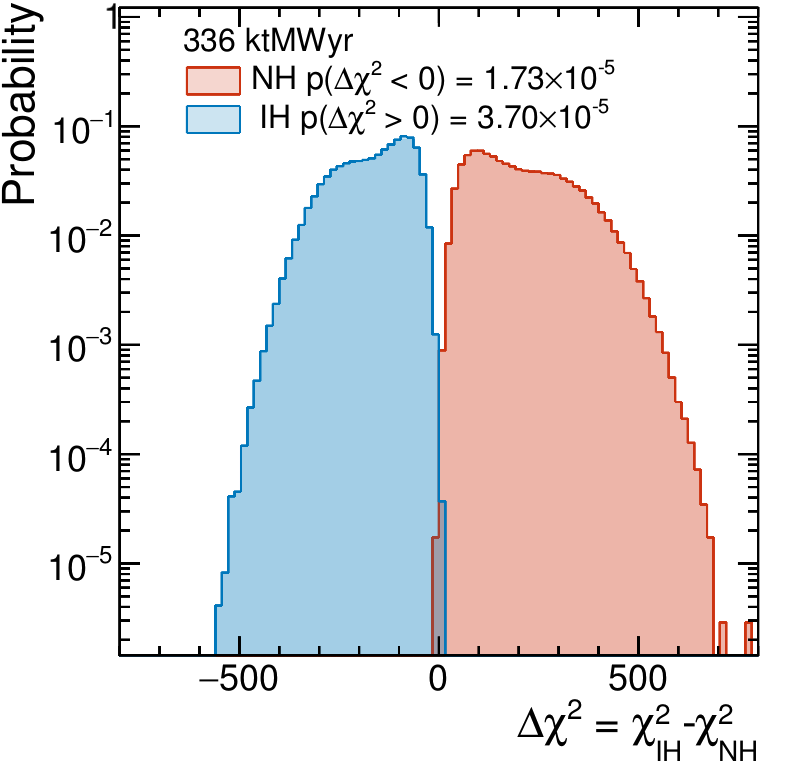
\includegraphics[width=0.33\linewidth]{MH_comp_ndfd_336ktMWyr_th13.png}}
  \caption{The distribution of $\dchisqMO = \chi^{2}_{\mathrm{IO}} - \chi^{2}_{\mathrm{NO}}$ values shown for both true normal (red) and true inverted (blue) hierarchies built using random throws of the systematic parameters, the oscillation parameters and with statistical variations. In each case, the $\chi^{2}$ values are separately minimized with respect to all variable parameters before calculating the test statistic. The fraction of throws for which the value of \dchisqMO is greater than (less than) 0 is also given for inverted (normal) hierarchies. For each ordering and exposure, approximately 100,000 throws were used.}
  \label{fig:mh_comp_over_time}
\end{figure*}
Given the complications with the interpretation of significance for mass ordering determination, it is instructive to look at the distribution of the test-statistic (Equation~\ref{eq:mh_chi2}), which gives more information than the 68\% central band and median throw shown in Figure~\ref{fig:mh_bands}. Figure~\ref{fig:mh_comp_over_time} shows the distribution of \dchisqMO obtained for a large ensemble of throws, for both true normal and inverted orderings, for a number of different exposures. There is a uniform distribution of true \deltacp used in the throws at each exposure. The change in shape at higher exposures in Figure~\ref{fig:mh_comp_over_time} is due to the degeneracy between \deltacp and the effect of the mass ordering, and as might be expected from Figure~\ref{fig:mh_bands}, the separation between hierarchies is greater for some true values of \deltacp than others. This additional structure starts to become obvious from a $\approx$66 kt-MW-yr exposure, at which point the CPV sensitivity is not very strong (see Section~\ref{sec:cp_sens}). For all exposures, the shape of the throw distribution is highly non-Gaussian, which makes it difficult to apply simple corrections to the sensitivity of the sort described in Ref.~\cite{Blennow:2013oma}. As a result alternatives to $\sqrt{\dchisqMO}$ as a sensitivity metric are not explored, the full information is given in Figure~\ref{fig:mh_comp_over_time}.

\begin{figure}[htbp]
  \centering
  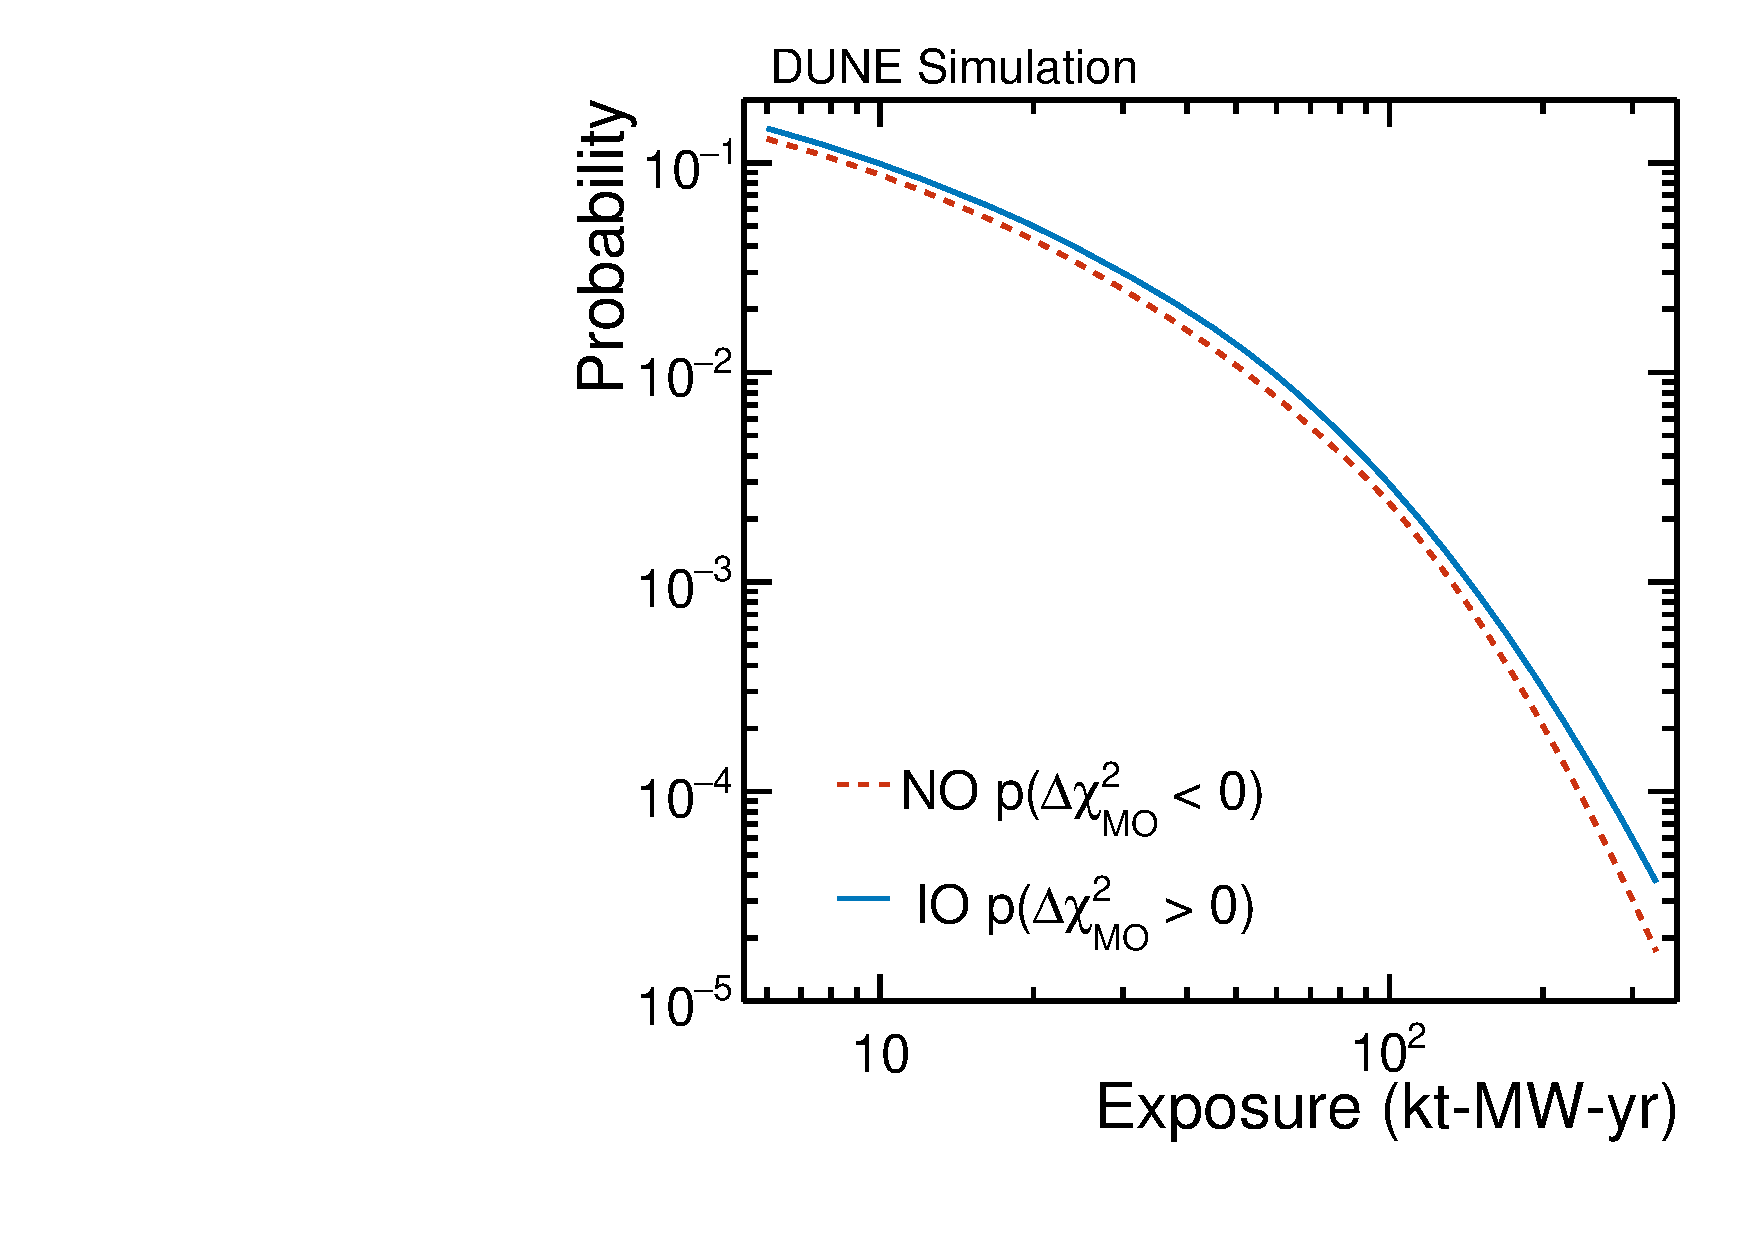
\includegraphics[width=0.8\linewidth]{fraction_throws_vs_exp_wrong_ordering.pdf}
  \caption{The probability for preferring the wrong neutrino mass ordering as a function of exposure, shown for both true NO and IO.}
  \label{fig:mh_wrong}
\end{figure}
Figure~\ref{fig:mh_comp_over_time} also indicates the probability for the test statistic \dchisqMO to be less (more) than zero from the toy throws for true normal (inverted) orderings at each exposure. This information is summarized in Figure~\ref{fig:mh_wrong}. This marks the proportion of toys which appear more like the incorrect ordering than the true ordering for the toy, and gives a sense of the ambiguity between the hierarchies, although it is not easily converted to a single number sensitivity. It is clear from Figures~\ref{fig:mh_comp_over_time} and~\ref{fig:mh_wrong} that DUNE is sensitive to the mass ordering even from very low ($\approx$12 kt-MW-yr) exposures, with a small probability for preferring the incorrect ordering. By exposures of 66 kt-MW-yr, the overlap between the orderings is very small with $\approx$1\% of toy throws which appear more like the incorrect ordering than the true ordering.

\begin{figure*}[htbp]
  \centering
  \subfloat[6 kt-MW-yr]   {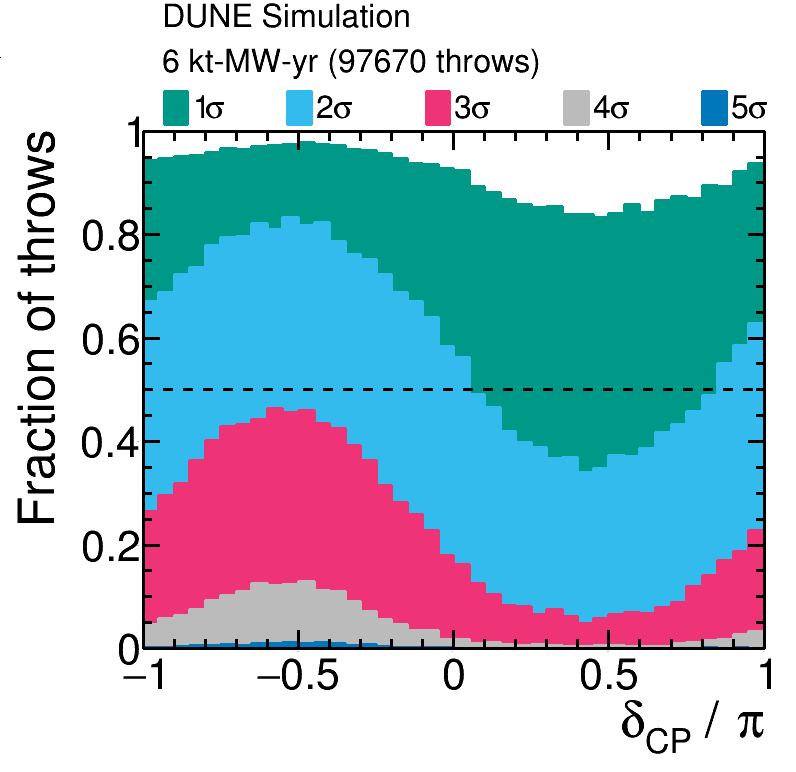
\includegraphics[width=0.33\linewidth]{mh_throws_6ktMWyr_NH_th13.png}}
  \subfloat[12 kt-MW-yr]  {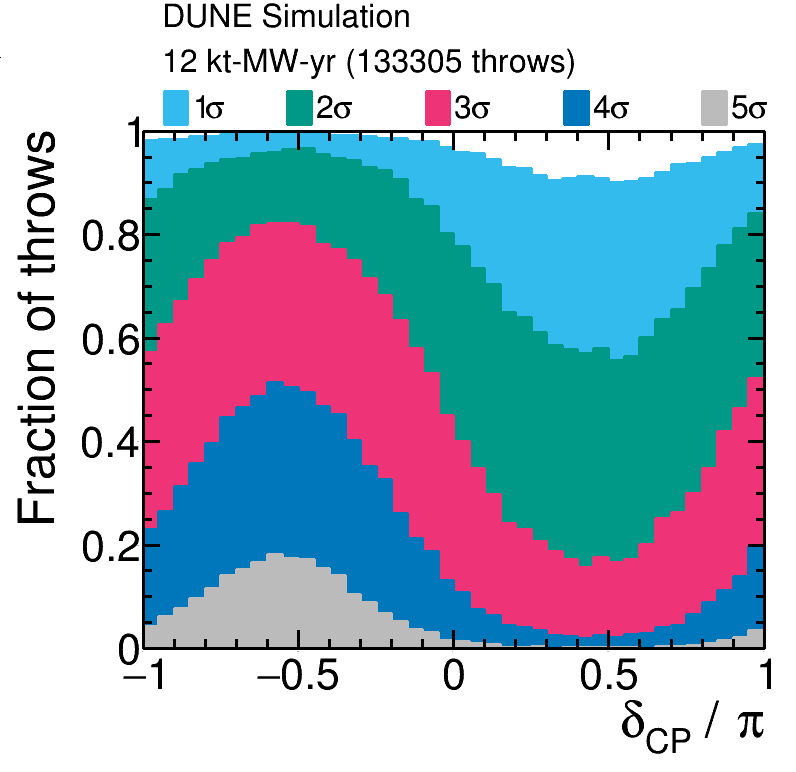
\includegraphics[width=0.33\linewidth]{mh_throws_12ktMWyr_NH_th13.png}}
  \subfloat[24 kt-MW-yr]  {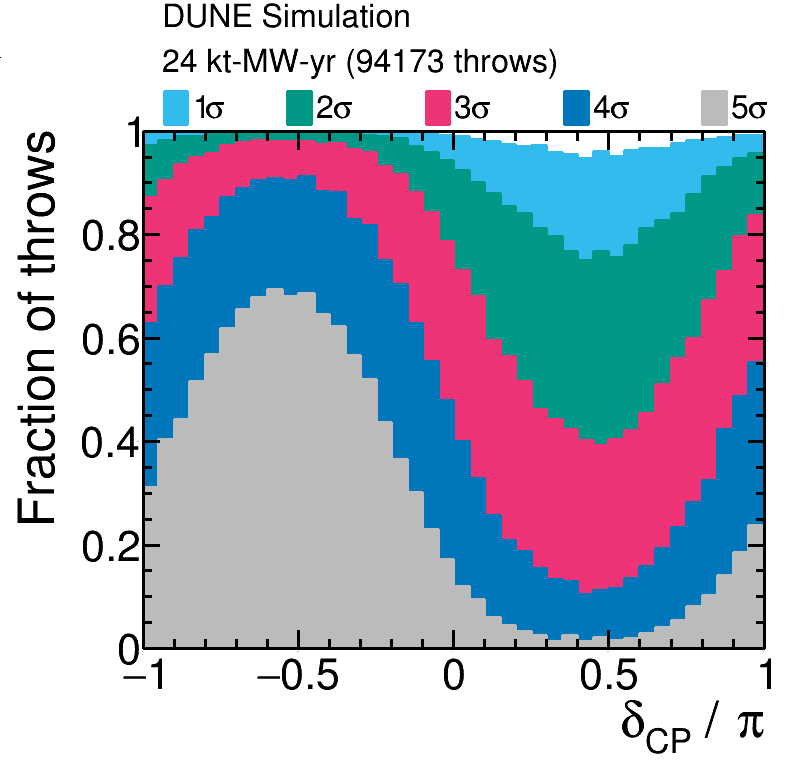
\includegraphics[width=0.33\linewidth]{mh_throws_24ktMWyr_NH_th13.png}}\\
  \subfloat[66 kt-MW-yr]  {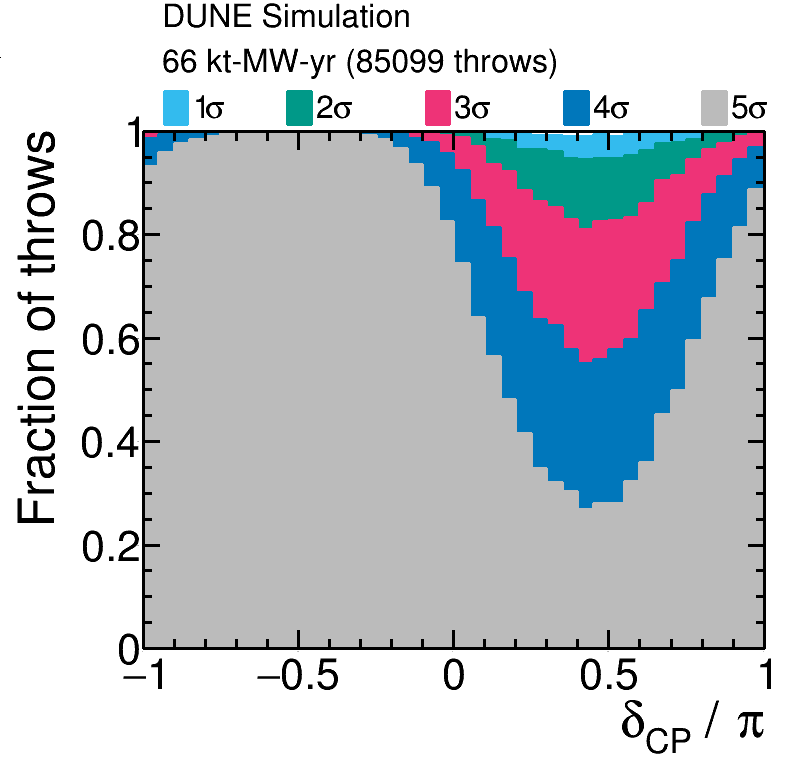
\includegraphics[width=0.33\linewidth]{mh_throws_66ktMWyr_NH_th13.png}}
  \subfloat[100 kt-MW-yr] {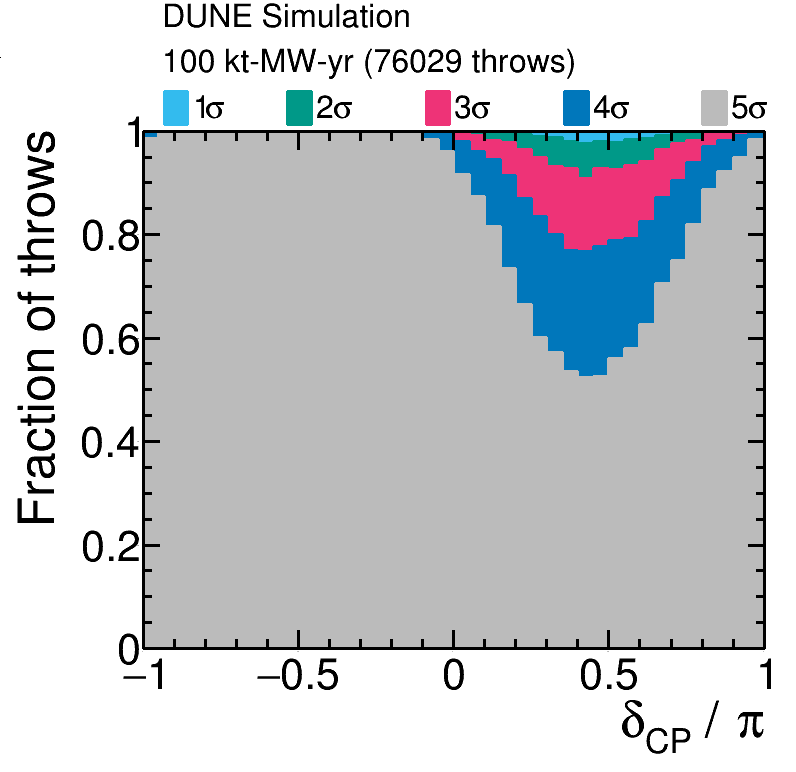
\includegraphics[width=0.33\linewidth]{mh_throws_100ktMWyr_NH_th13.png}}
  \subfloat[336 kt-MW-yr] {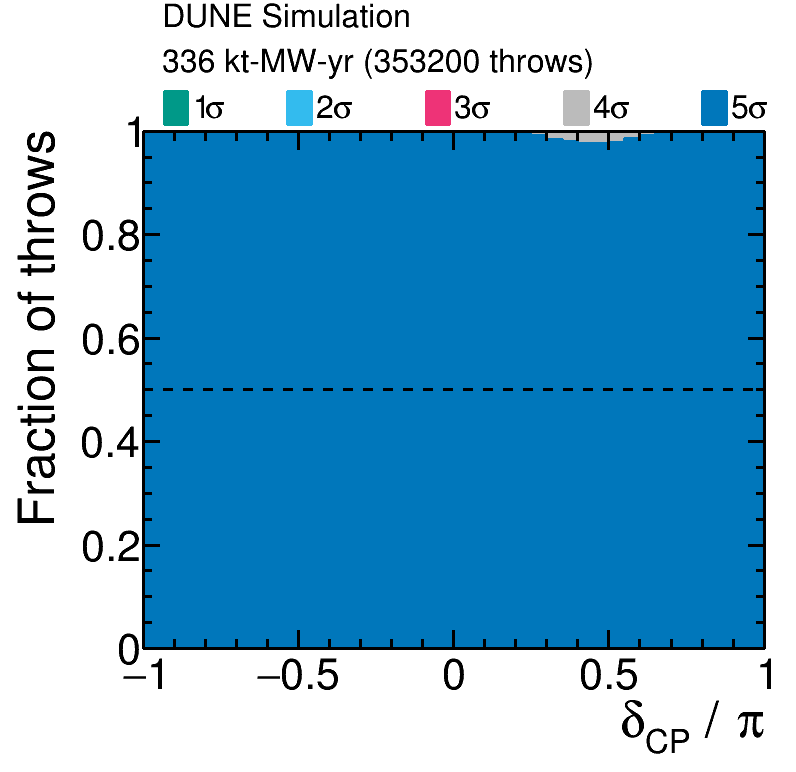
\includegraphics[width=0.33\linewidth]{mh_throws_336ktMWyr_NH_th13.png}}
  \caption{Fraction of throws for which the DUNE sensitivity to the mass ordering exceeds 1--5$\sigma$ significance, as a function of the true value of \deltacp. Shown for NO, for a number of different exposures. The number of throws used to make each figure is also shown.}
  \label{fig:mh_nh_over_time}
\end{figure*}

Figure~\ref{fig:mh_nh_over_time} shows an alternative way to present the result of the throws as a function of \deltacp, which is complementary to Figure~\ref{fig:mh_bands}. The fraction of throws for which the simple figure of merit (the square-root of Equation~\ref{eq:mh_chi2}) exceeds different confidence levels are shown, for 1--5$\sigma$ significances, and a variety of exposures, all for true NO. The same throws are used as in Figures~\ref{fig:mh_comp_over_time}. Despite the caveats regarding the intepretation of $\sqrt{\dchisqMO}$ as units of $\sigma$, the general trend is clear, and provides more information about the expected DUNE sensitivity at low exposures. As with Figures~\ref{fig:cpv_over_time_fc} and~\ref{fig:cpv_over_time}, the point at which the median significance (50\% of throws) passes different significance thresholds can be easily read from the figures, and can be compared with those shown in Figure~\ref{fig:mh_bands}. The same general shape as a function of \deltacp as was observed in Figure~\ref{fig:mh_bands} can be seen. The general trend would be very similar in IO, reflected in the line $\deltacp = 0$, although a slightly longer exposure is required to reach the same sensitivity. The median significance for $\deltacp = -\pi/2$ exceeds 5$\sigma$ for 24 kt-MW-yr, at which point the fraction of throws for which the significance is 3$\sigma$ or smaller is only $\approx$2\%. By 66 kt-MW-yr, 100\% of the throws exceed 5$\sigma$ at $\deltacp = -\pi/2$. By 100 kt-MW-yr exposures, the median significance approaches 5 $\sigma$ for all true values of \deltacp. At long exposures of 336 kt-MW-yr, almost 100\% of the throws exceed 5$\sigma$ for all values of \deltacp.
